\documentclass[12pt]{article}

\usepackage{sbc-template}
\usepackage[brazil,american]{babel}
\usepackage[utf8]{inputenc}

\usepackage{graphicx}
\usepackage{url}
\usepackage{float}
\usepackage{listings}
\usepackage{color}
\usepackage{todonotes}
\usepackage{algorithmic}
\usepackage{algorithm}
\usepackage{hyperref}
\usepackage{amssymb}
\usepackage{amsmath}
\usepackage{enumitem}
\graphicspath{{../parte1/graficos/}{../parte2/graficos/}}

\sloppy

\title{Trabalho 2\\
Ajuste de Curvas\\
\& \\
Splines}

\author{Dayanne Fernandes da Cunha, 13/0107191\\
       Yurick Hauschild, 12/0024136\\
       Grupo 6
}

\address{Dep. Matemática $-$ Universidade de Brasília (UnB)\\
  Cálculo Numérico $-$ Turma A
  \email{dayannefernandesc@gmail.com, yurick.hauschild@gmail.com}
}

\begin{document}
\maketitle

\selectlanguage{brazil}

 \begin{resumo}
 	Este relatório corresponde aos informativos das resoluções do Trabalho 2 de Cálculo Numérico da Turma A do semestre 2016/2.
 \end{resumo}

\section{Parte I : Ajuste de Curvas}
\label{sec:parte1}

Esta primeira parte de trabalho será dedicada aos ajustes de curvas pelo método dos mínimos quadrados. Para tal, considere o conjunto de dados apresentado na Figura~\ref{fig:tab1}.

\begin{figure}[H]
	\centering
	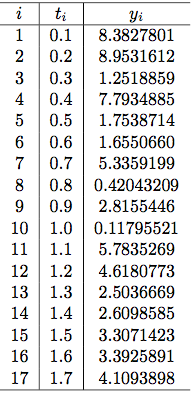
\includegraphics[width=0.3\textwidth]{tab1.png}
	\caption{Tabela de pontos.}
	\label{fig:tab1}
\end{figure}

\subsection{Questão 1}
\label{subsec:p1q1}

Determine, para o conjunto de pontos da Figura~\ref{fig:tab1}, os melhores ajustes polinomiais de grau 1, 2, 3, 5 e 10. Trace os seus resultados e comente sobre a adequação de cada um destes ajustes. É possível encontrar uma maneira quantitativa de se julgar qual dentre estes cinco ajustes é o melhor?

\textbf{Resolução:}

O método dos quadrados mínimos foi implementado e pode ser encontrado no arquivo '$\textbf{parte1/q1.f90}$'. A partir dele, foi possível encontrar os seguintes ajustes:

\begin{gather*}
    y_{1} = 5.4491559 - 1.819038x \\
    y_{2} = 8.7060667 - 12.10402x + 5.7138785x^{2} \\
    y_{3} = 11.099895 - 26.10301x + 24.612525x^{2} - 6.999498x^{3} \\
    y_{5} = 11.820173 - 30.99526x + 29.737760x^{2} - 0.489529x^{3} - 10.879890x^{4} + 3.668555x^{5} \\
    y_{10} = 10.767245 - 21.21473x + 8.5667448x^{2} + 7.315704x^{3} + 0.6093679x^{4} - 1.894178x^{5} - \\ 1.310241x^{6} - 0.297909x^{7} + 0.1513477x^{8} + 0.159235x^{9} + 0.025067x^{10}
\end{gather*}

Cada um deles está representado graficamente e podem ser encontrados nos arquivos '\textbf{parte1/graficos/q1.1.png}', '\textbf{parte1/graficos/q1.2.png}', '\textbf{parte1/graficos/q1.3.png}', '\textbf{parte1/graficos/q1.5.png}' e '\textbf{parte1/graficos/q1.10.png}', respectivamente.
É fácil de verificar pelos gráficos que nenhum dos ajustes realmente cobriu perfeitamente os pontos da tabela, mas dada a grande discrepância entre vários valores muitas vezes consecutivos, isto é um comportamento bastante compreensível.

Utilizando-se do coeficiente de determinação $R^{2}$, é possível mensurar a adequação de cada um destes ajustes e, por conseguinte, decidir qual dentre eles é o melhor.

O coeficiente $R^{2}$ é calculado a partir da fórmula

\begin{equation}
    R^{2} = 1 - \frac{SQ_{err}}{SQ_{tot}}
\end{equation}

Onde $SQ_{err}$ é a soma dos quadrados dos erros e ${SQ_{tot}}$ é a soma dos quadrados total.

Temos, então, o resultado:

\begin{itemize}[noitemsep]
\item 71,9055769\% da variância de $y_{1}$ é explicada pela tabela;
\item 78,8906477\% da variância de $y_{2}$ é explicada pela tabela;
\item 80,7774013\% da variância de $y_{3}$ é explicada pela tabela;
\item 81,0324401\% da variância de $y_{5}$ é explicada pela tabela;
\item 81,3383318\% da variância de $y_{10}$ é explicada pela tabela.
\end{itemize}

Concluímos, então, que $y_{10}$, dentre os ajustes calculados, é o que melhor aproxima a função proposta na tabela.
Por outro lado, é notável que a melhora entre $y_{5}$ e $y_{10}$ foi mínima.

\subsection{Questão 2}
\label{subsec:p1q2}

Encontre o polinômio interpolador para estes dados e trace o seu resultado num gráfico. Apresente, igualmente, o polinômio interpolador encontrado teoricamente, usando polinômios de Lagrange (talvez seja recomendado usar algum programa de manipulação simbólica!). Comente seus resultados. Se você precisasse de uma função para descrever os dados da tabela, qual dentre o polinômio interpolador e os ajustes encontrados na questão 1 você escolheria? Por quê?

\textbf{Resolução:}

Para tentar ajustar os pontos da Figura~\ref{fig:tab1} foi utilizado o método de mínimos quadrados na questão 1, já nesta questão foi requisitado que ajustasse a curva utilizando o polinômio interpolador utilizando polinômios de Lagrange.

Para uma determinada função $f(x)$ se tivermos n+1 pontos $(x_{i}, y_{i})$ com $t_{i} \neq t_{j}$ $\forall i,j$ sempre encontraremos um único polinômio interpolador de grau menor ou igual a $n$ tal que $y(x_{i}) = y_{i} \forall i=1,..,n+1$.

Logo, no nosso exemplo da Figura~\ref{fig:tab1} iremos encontrar um polinômio interpolador de grau menor ou igual a $n = 16$ do formato apresentado na Equação~\ref{eq:polinter}.

\begin{eqnarray}
\begin{split}
P(t) = \alpha_{1} + \alpha_{2}t + ... + \alpha_{n+1}t^{n}
\end{split}
\label{eq:polinter}
\end{eqnarray}

Após manipulação do sistema linear apresentado na Equação~\ref{eq:polinter} podemos chegar a uma expressão mais elegante para representar o polinômio interpolador, por polinômios de Lagrange (Equação~\ref{eq:lagrange}).

\begin{eqnarray}
\begin{split}
\mathcal{L}_{i}(t) = \prod_{1 \leq k \leq n+1,  k \neq i} \dfrac{(t - t_{k})}{(t_{i} - t_{k})}
\end{split}
\label{eq:lagrange}
\end{eqnarray}

Na Equação~\ref{eq:lagrange} sendo $i = 1,..,n+1$ e $k = 1, .., n+1$, tal que, $k \neq i$. Com o polinômio de Lagrange podemos aproximar qualquer distribuição de pontos além de, por propriedade do polinômio interpolador, a de passar exatamente em todos os pontos $(x_{i}, y_{i})$, o erro do ajuste é \textbf{nulo} ($\mathcal{E}\equiv 0$)! 

Com os polinômio de Lagrange podemos construir uma nova expressão para o polinômio interpolador, que denominaremos por \textbf{Polinômio Interpolador de Lagrange} $P(t)$ de $n+1$ pontos como é mostrado na Equação~\ref{eq:polinterlagrange}.

\begin{eqnarray}
\begin{split}
P_{i}(t) = y_{1}\mathcal{L}_{1}(t) + y_{2}\mathcal{L}_{2}(t) + ... + y_{n+1}\mathcal{L}_{n+1}(t) = \sum^{n+1}_{k=1} y_{k}\mathcal{L}_{k}(t)
\end{split}
\label{eq:polinterlagrange}
\end{eqnarray}

Na nossa Questão~\ref{subsec:p1q2} utilizando o algoritmo implementado no arquivo '\textbf{parte1/q2.f90}' foi possível encontrar um Polinômio Interpolador de Lagrange utilizando os 17 ponto da tabela da Figura~\ref{fig:tab1}, o gráfico encontrado está apresentado na Figura~\ref{fig:p1q2}.

\begin{figure}[H]
	\centering
	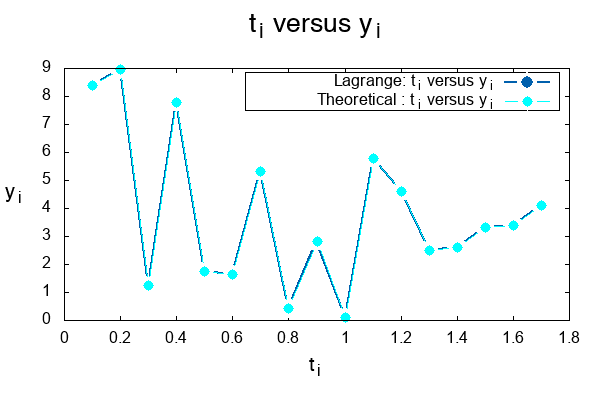
\includegraphics[width=0.6\textwidth]{p1q2g1.png}
	\caption{Gráfico de número de pontos $t_{i}$ a cada $y_{i}$.}
	\label{fig:p1q2}
\end{figure}

Foi implementado outro algoritmo de nome '\textbf{parte1/assistq2.cc}' para encontrar o valor teórico do Polinômio Interpolador de Lagrange devido à extensão da quantidade de pontos. Sendo os polinômios de Lagrange apresentados nas equações abaixo:

\begin{gather*}
	\displaybreak 
	\mathcal{L}_{1}(t) = 477.947733*t^{16} + -7264.805545*t^{15} + 50949.228363*t^{14} + \\ -218670.646911*t^{13} +  642316.921975*t^{12} + -1367942.542711*t^{11} + \\ 2182792.564685*t^{10} + -2659094.855792*t^{9} +  2496269.449097*t^{8} + \\ -1809422.218701*t^{7} + 1007801.986291*t^{6} + -426054.256882*t^{5} + \\ 133763.333550*t^{4} + -30083.449528*t^{3} + 4559.068304*t^{2} + \\ -414.723929*t + 17.000000 \\ \\
	\mathcal{L}_{2}(t) = -7647.163732*t^{16} + 115472.172350*t^{15} + -803716.908214*t^{14} + \\ 3419505.734321*t^{13} +  -9943042.639802*t^{12} + 20926179.230577*t^{11} + \\ -32928153.257188*t^{10} + 39452355.144733*t^{9} + -36304391.925880*t^{8} + \\ 25683908.232596*t^{7} +  -13883125.684062*t^{6} + 5652726.151367*t^{5} + \\ -1691354.917535*t^{4} + 357085.542625*t^{3} +  -49661.503588*t^{2} + \\ 3997.791431*t + -136.000000 \\ \\
	\mathcal{L}_{3}(t) = 57353.727989*t^{16} + -860305.919830*t^{15} + 5942993.294184*t^{14} + \\ -25068970.381470*t^{13} + 72181387.285554*t^{12} + -150206492.003367*t^{11} + \\ 233288470.673763*t^{10} +  -275298352.269148*t^{9} + 248871966.480458*t^{8} + \\ -172424309.689153*t^{7} + 90922012.072611*t^{6} +  -35943531.039562*t^{5} + \\ 10381191.796691*t^{4} + -2100816.406981*t^{3} + 277844.668751*t^{2} + \\ -21122.290487*t + 680.000000 \\ \\
	\mathcal{L}_{4}(t) = -267650.730614*t^{16} + 3987995.886144*t^{15} + -27343198.639495*t^{14} + \\ 114371439.602921*t^{13} + -326194456.692142*t^{12} + 671539788.871965*t^{11} + \\ -1030352703.066824*t^{10} + 1199188421.639232*t^{9} + -1067144834.763252*t^{8} + \\ 726209597.716723*t^{7} + -375212917.483644*t^{6} + 144942128.092822*t^{5} + \\ -40789653.936149*t^{4} + 8021616.840154*t^{3} + -1029104.687882*t^{2} + \\ 75911.350039*t + -2380.000000 \\ \\
	\mathcal{L}_{5}(t) = 869864.874495*t^{16} + -12874000.142519*t^{15} + 87612790.159087*t^{14} + \\ -363446941.861294*t^{13} + 1027091384.802612*t^{12} + -2093011415.132366*t^{11} + \\ 3175142302.934550*t^{10} + -3649249732.847102*t^{9} + 3202540794.688023*t^{8} + \\ -2146199080.427569*t^{7} + 1090414918.639800*t^{6} + -413631249.710509*t^{5} + \\ 114175516.957898*t^{4} + -22009046.368547*t^{3} + 2768168.943543*t^{2} + \\ -200463.510101*t + 6188.000000 \\ \\  \displaybreak
	\mathcal{L}_{6}(t) = -2087675.698787*t^{16} + 30688832.772166*t^{15} + -207306196.889530*t^{14} + \\ 853024290.524290*t^{13} + -2389341079.445246*t^{12} + 4822132410.413660*t^{11} + \\ -7238675778.953555*t^{10} + 8225164654.982363*t^{9} + -7130098793.678349*t^{8} + \\ 4715867470.444774*t^{7} + -2362914218.981731*t^{6} + 883464370.283940*t^{5} + \\ -240300118.181200*t^{4} + 45652260.725269*t^{3} + -5663104.671597*t^{2} + \\ 405052.353535*t + -12376.000000 \\ \\
	\mathcal{L}_{7}(t) = 3827405.447776*t^{16} + -55880119.537527*t^{15} + 374702993.337252*t^{14} + \\ -1529622587.203604*t^{13} + 4248049554.183809*t^{12} +  -8495216585.219469*t^{11} + \\ 12628599636.549564*t^{10} + -14201992145.398521*t^{9} + 12178134407.111917*t^{8} + \\ -7964171617.216579*t^{7} + 3944543486.904145*t^{6} + -1457709878.900890*t^{5} + \\ 391964108.747244*t^{4} + -73651065.205908*t^{3} + 9044099.718254*t^{2} + \\ -641141.317460*t + 19448.000000 \\ \\
	\mathcal{L}_{8}(t) = -5467722.068251*t^{16} + 79281969.989642*t^{15} + -527744534.027602*t^{14} + \\ 2137682490.691748*t^{13} + -5888118814.912789*t^{12} + 11673578195.424250*t^{11} + \\ -17197210652.522308*t^{10} + 19159391322.243896*t^{9} + -16271813954.906149*t^{8} + \\ 10538071267.782116*t^{7} + -5168776727.139668*t^{6} + 1891964789.336541*t^{5} + \\ -504086774.213435*t^{4} + 93910496.813508*t^{3} + -11442810.209751*t^{2} + \\ 805767.718254*t + -24310.000000 \\ \\
	\mathcal{L}_{9}(t) = 6151187.326783*t^{16} + -88577097.505669*t^{15} + 585346986.016629*t^{14} + \\ -2353050595.238094*t^{13} + 6430302372.685184*t^{12} +  -12644810267.857141*t^{11} + \\ 18472753118.898018*t^{10} + -20406327017.786274*t^{9} + 17183548573.281303*t^{8} + \\ -11034769019.717260*t^{7} + 5367845841.290509*t^{6} + -1949298185.267857*t^{5} + \\ 515497564.651931*t^{4} + -95379597.520550*t^{3} + 11550970.849632*t^{2} + \\ -809144.107143*t + 24310.000000 \\ \\
	\mathcal{L}_{10}(t) = -5467722.068251*t^{16} + 78188425.575992*t^{15} + -512981684.443324*t^{14} + \\ 2046896433.470506*t^{13} + -5551368373.995686*t^{12} + 10832704873.358803*t^{11} + \\ -15703368335.502916*t^{10} + 17213791508.758846*t^{9} + -14385535503.942440*t^{8} + \\ 9169986927.764606*t^{7} + -4429246813.600760*t^{6} + 1597739357.447518*t^{5} + \\ -419919248.235150*t^{4} + 77260667.949106*t^{3} + -9310539.711451*t^{2} + \\ 649476.174603*t + -19448.000000 \\ \\
	\mathcal{L}_{11}(t) = 3827405.447776*t^{16} + -54349157.358417*t^{15} + 354035003.919263*t^{14} + \\ -1402476178.228493*t^{13} + 3776061569.174994*t^{12} + -7315183547.055652*t^{11} + \\ 10528549344.441994*t^{10} + -11460607612.097050*t^{9} + 9512860535.584154*t^{8} + \\ -6024719113.052370*t^{7} + 2892272594.598153*t^{6} + -1037390465.675828*t^{5} + \\ 271231511.734458*t^{4} + -49671278.421076*t^{3} + 5961439.099206*t^{2} + \\ -414428.111111*t + 12376.000000 \\ \\ \displaybreak
	\mathcal{L}_{12}(t) = -2087675.698787*t^{16} + 29436227.352894*t^{15} + -190396023.729357*t^{14} + \\ 748932780.182781*t^{13} + -2002436317.540486*t^{12} + 3852813477.032231*t^{11} + \\ -5508579052.763086*t^{10} + 5958075259.038807*t^{9} + -4915507275.821213*t^{8} + \\ 3095318015.666339*t^{7} + -1478053082.448995*t^{6} + 527549202.734188*t^{5} + \\ -137319697.070540*t^{4} + 25048695.149341*t^{3} + -2996026.927549*t^{2} + \\ 207682.843434*t + -6188.000000 \\ \\
	\mathcal{L}_{13}(t) = 869864.874495*t^{16} + -12178108.242923*t^{15} + 78218249.514546*t^{14} + \\ -305569612.571927*t^{13} + 811574359.389753*t^{12} + -1551510440.326992*t^{11} + \\ 2204684438.075642*t^{10} + -2370731114.816041*t^{9} + 1945215211.850720*t^{8} + \\ -1218689702.365643*t^{7} + 579217845.778247*t^{6} + -205855509.518688*t^{5} + \\ 53378979.438858*t^{4} + -9704131.576980*t^{3} + 1157321.077742*t^{2} + \\ -80030.580808*t + 2380.000000 \\ \\
	\mathcal{L}_{14}(t) = -267650.730614*t^{16} + 3720345.155530*t^{15} + -23729913.776210*t^{14} + \\ 92086839.772025*t^{13} + -243021456.852476*t^{12} + 461787531.955357*t^{11} + \\ -652466073.878112*t^{10} + 697876999.436607*t^{9} + -569792404.207697*t^{8} + \\ 355358165.731249*t^{7} + -168195324.546585*t^{6} + 59553840.721061*t^{5} + \\ -15391128.163792*t^{4} + 2789898.985305*t^{3} + -331892.844517*t^{2} + \\ 22903.242868*t + -680.000000 \\ \\
	\mathcal{L}_{15}(t) = 57353.727989*t^{16} + -791481.446243*t^{15} + 5013862.900768*t^{14} + \\ -19331074.018574*t^{13} + 50705467.372134*t^{12} + -95802707.130832*t^{11} + \\ 134646357.578525*t^{10} + -143315357.103489*t^{9} + 116488436.505968*t^{8} + \\ -72353244.874339*t^{7} + 34119437.667849*t^{6} + -12040978.159572*t^{5} + \\ 3102783.869202*t^{4} + -560998.142186*t^{3} + 66592.377566*t^{2} + \\ -4587.124764*t + 136.000000 \\ \\
	\mathcal{L}_{16}(t) = -7647.163732*t^{16} + 104766.143126*t^{15} + -659185.513683*t^{14} + \\ 2525552.294071*t^{13} + -6586060.116153*t^{12} + 12377091.572693*t^{11} + \\ -17310042.586994*t^{10} + 18341917.656980*t^{9} + -14847794.703658*t^{8} + \\ 9188315.091919*t^{7} + -4318603.183511*t^{6} + 1519586.194562*t^{5} + \\ -390562.236508*t^{4} + 70456.947719*t^{3} + -8347.495762*t^{2} \\ + 574.098929*t + -17.000000 \\ \\
	\mathcal{L}_{17}(t) = 477.947733*t^{16} + -6500.089172*t^{15} + 40625.557325*t^{14} + \\ -154702.122295*t^{13} + 401190.378766*t^{12} + -750150.591007*t^{11} + \\ 1044330.814244*t^{10} + -1102011.728045*t^{9} + 888758.997000*t^{8} + \\ -548158.868711*t^{7} + 256874.131353*t^{6} + -90148.432211*t^{5} + \\ 23116.424479*t^{4} + -4161.861269*t^{3} + 492.249100*t^{2} \\ + -33.807290*t + 1.000000
\label{eq:degreelagrange}
\end{gather*}

Portanto teremos o Polinômio Interpolador de Lagrange na equação abaixo, dados os $y_{i}$ da tabela da Figura~\ref{fig:tab1}.

\begin{gather*}
P_{i}(t) = 44929590.063424*t^{16} + -647280370.960326*t^{15} + 4279914865.346266*t^{14} + \\ -17217084770.868465*t^{13} + 47089293478.371513*t^{12} + -92686703619.757401*t^{11} + \\ 135548219756.010544*t^{10} + -149903217054.288818*t^{9} + 126370590293.072205*t^{8} + \\ -81237154218.415482*t^{7} + 39553248124.037933*t^{6} + -14372788603.944166*t^{5} + \\ 3802074486.481803*t^{4} + -703404093.061281*t^{3} + 85142565.074091*t^{2} + \\ -5959309.219498*t + 178882.175689
\label{eq:lagrangeq2}
\end{gather*}

Com o Polinômio Interpolador de Lagrange acima foi possível encontrar o \textbf{Fenômeno de Runge} como podemos ver na Figura~\ref{fig:runge} devido ao grau do polinômio ser alto.

\begin{figure}[H]
	\centering
	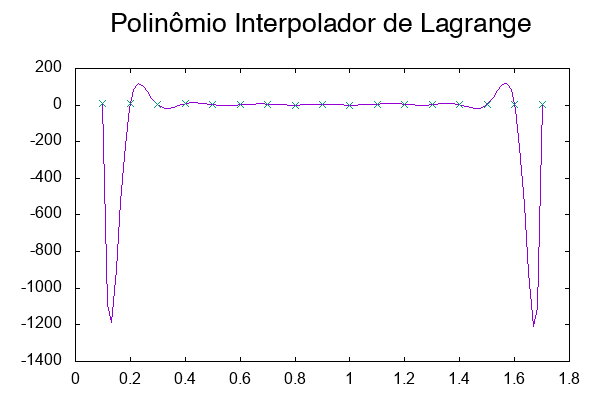
\includegraphics[width=0.6\textwidth]{p1q2g2.png}
	\caption{Gráfico do Fenômeno de Runge do Polinômio Interpolador de Lagrange utilizando a tabela da Figura~\ref{fig:tab1}.}
	\label{fig:runge}
\end{figure}

Utilizando o mesmo critério de avaliação do ajuste da curva apresentado na Questão~\ref{subsec:p1q1} foi também calculado para o Polinômio Interpolador de Lagrange, onde foi encontrado o seguinte resultado: $99.9997441$ \% da variância é explicada pela tabela. Logo podemos verificar numericamente que o Polinômio Interpolador de Lagrange mapeia quase $100$ \% dos dados na tabela da Figura~\ref{fig:tab1} sendo então este ajuste mais adequado para ser utilizado.

\subsection{Questão 3}
\label{subsec:p1q3}

\textbf{Resolução:}

\subsection{Questão 4}
\label{subsec:p1q4}

\textbf{Resolução:}

\section{Parte II : Splines}
\label{sec:parte2}

\subsection{Questão 5}
\label{subsec:p2q5}

\textbf{Resolução:}

\subsection{Questão 6}
\label{subsec:p2q6}

\textbf{Resolução:}

\subsection{Questão 7}
\label{subsec:p2q7}

\textbf{Resolução:}

\subsection{Questão 8}
\label{subsec:p2q8}

\textbf{Resolução:}

\subsection{Questão 9}
\label{subsec:p2q9}

\textbf{Resolução:}

\end{document}
